Just one more line to test github

 results with real data
 \begin{figure}[h]
    \centering
    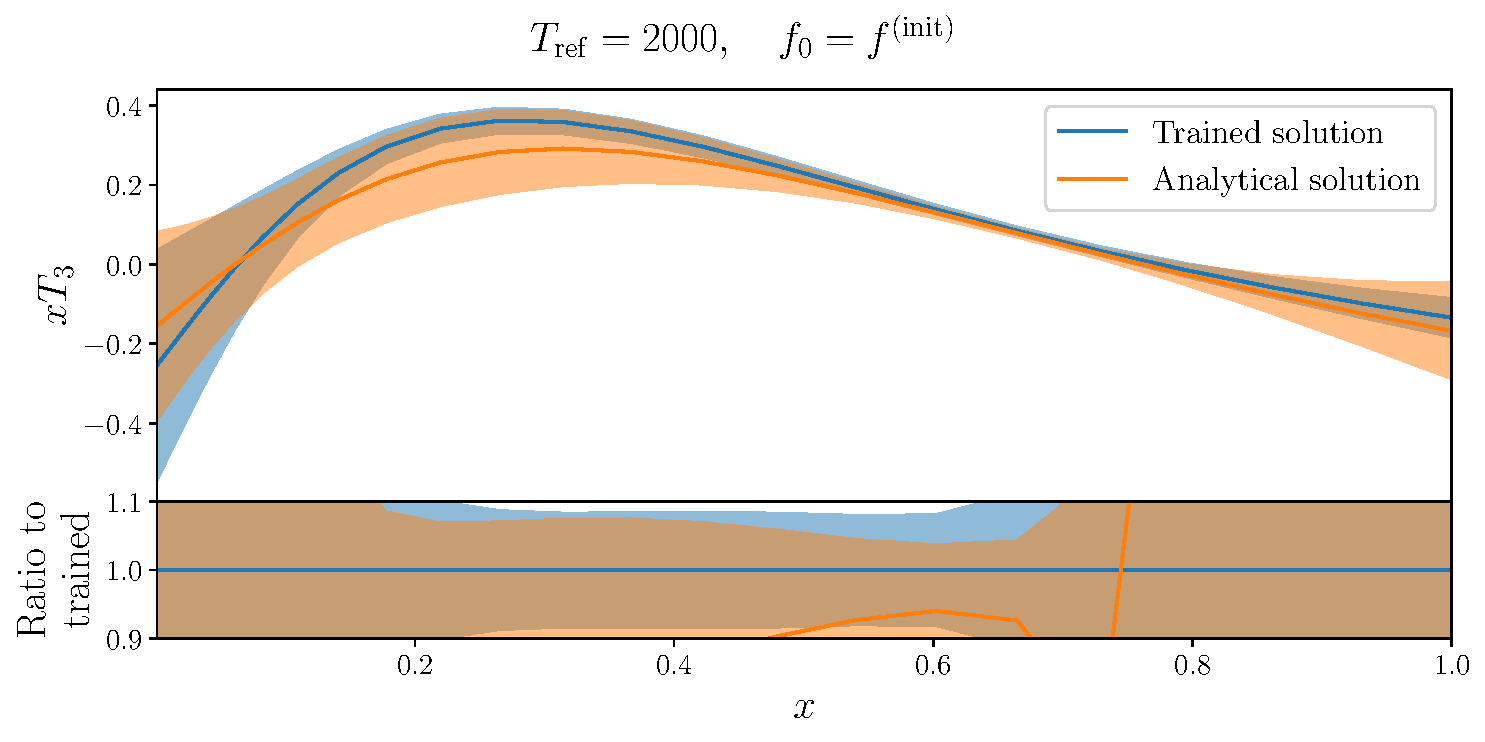
\includegraphics[width=0.48\textwidth]{plots/pdf_plot_init.pdf}
    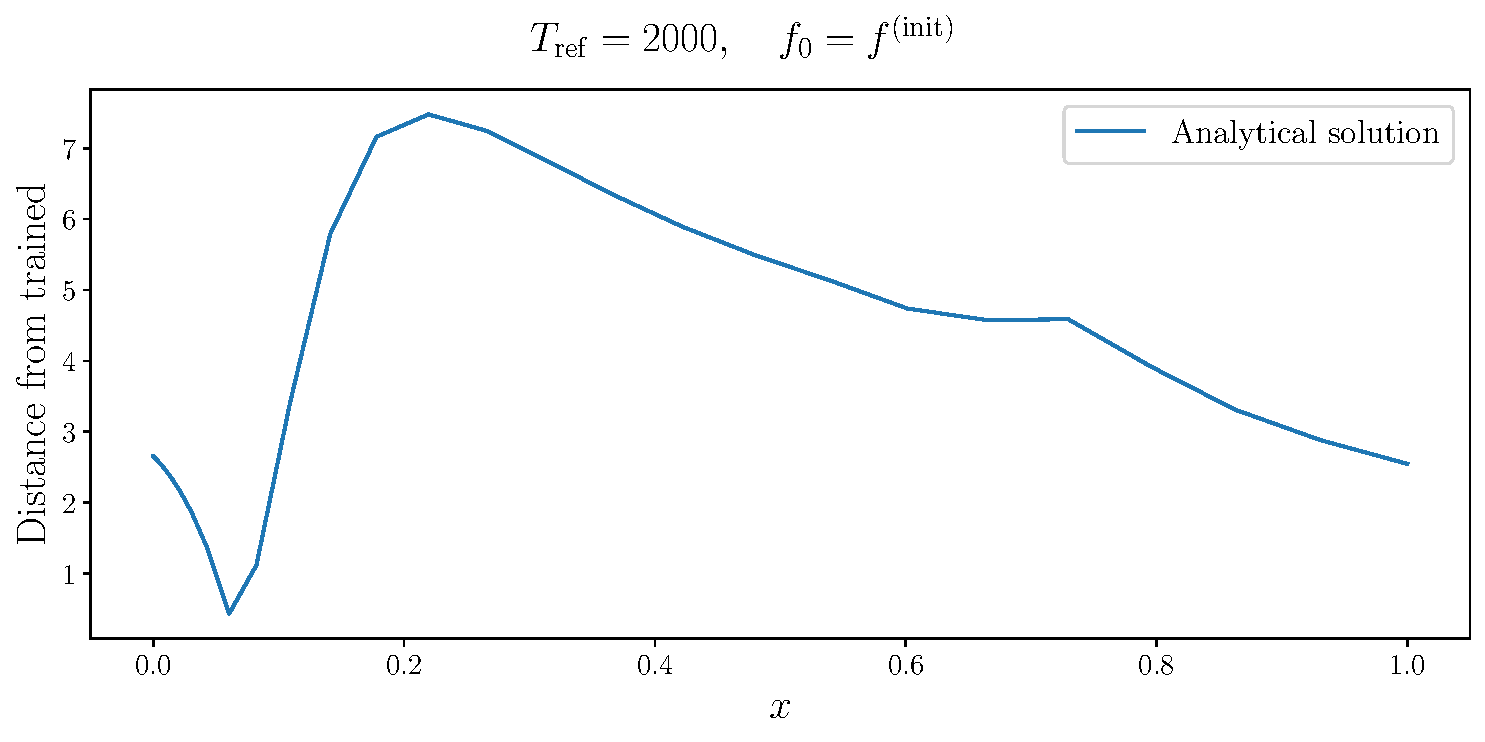
\includegraphics[width=0.48\textwidth]{plots/distance_plot_init.pdf}
    \caption{PDF comparison (left) and PDF distance (right) of the trained
    solution at the end of training (eot) and analytical solution. The frozen NTK
    is chosen at $T_{\rm ref} = 20000$ and the initial function $f_0$ is a
    different ensemble of networks at initialisation. The analytical solution is
    evolved for the equivalent of $T_{\rm tot}$ epochs. \ac{Plots obtained with L2
    data}}
    \label{fig:xT3_analytical_init}
  \end{figure}
  % ===================================
  
  % ===================================
  \begin{figure}[h]
    \centering
    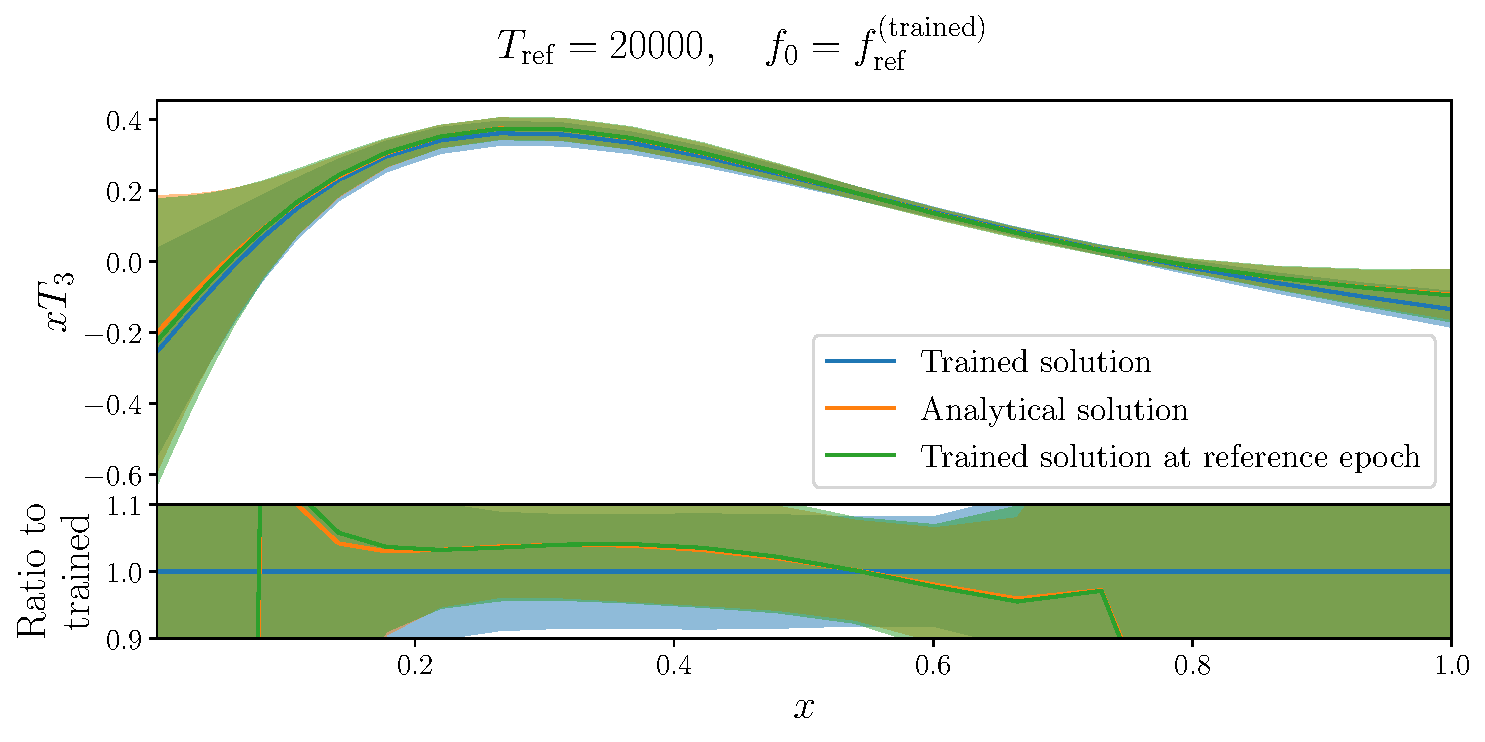
\includegraphics[width=0.48\textwidth]{plots/pdf_plot_ref_20000.pdf}
    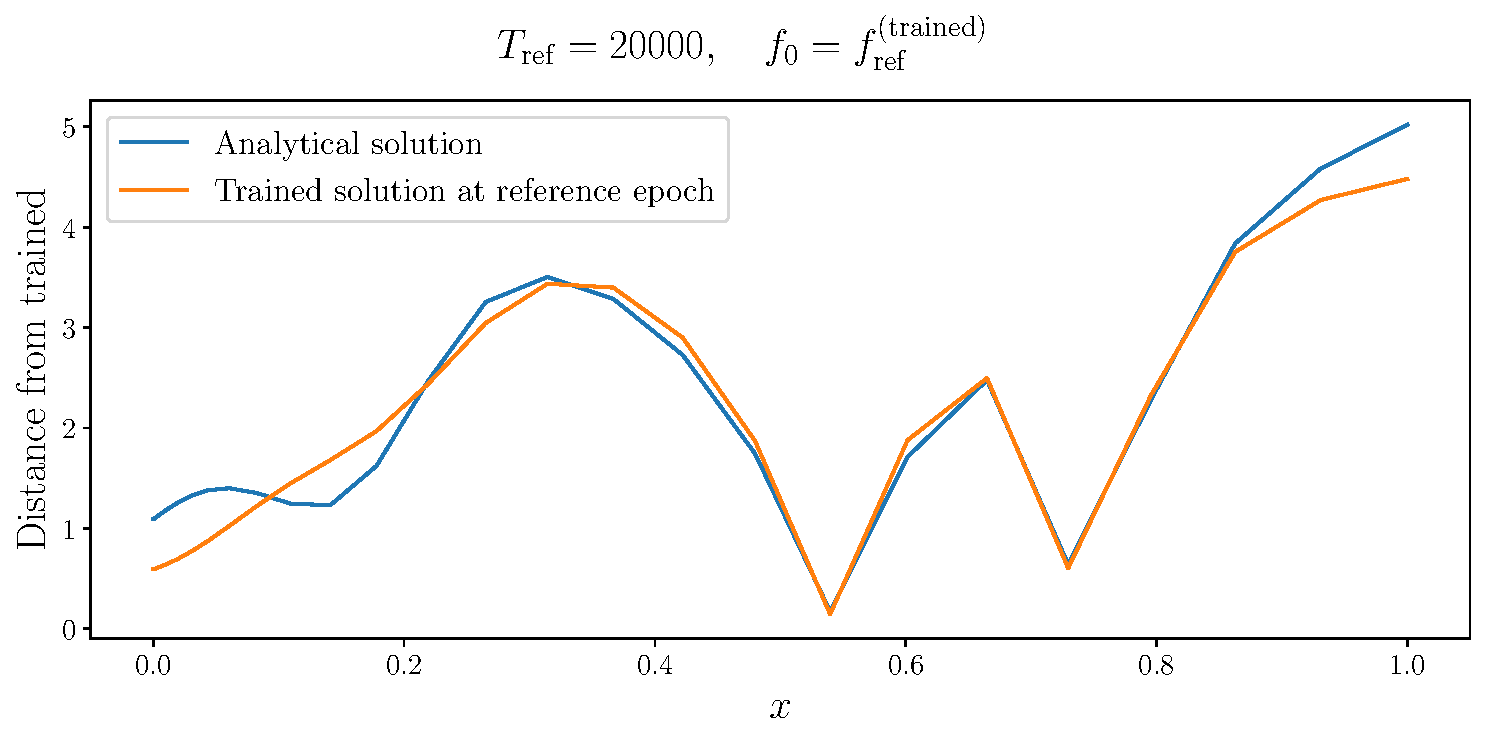
\includegraphics[width=0.48\textwidth]{plots/distance_plot_ref_20000.pdf}
    \caption{PDF comparison (left) and PDF distance (right) of the trained
    solution at the end of training (eot) and analytical solution. The frozen NTK
    is chosen at $T_{\rm ref} = 20000$ and the initial function $f_0$ is the
    trained function at $T_{\rm ref}$. The analytical solution is evolved for the
    equivalent of $T_{\rm tot} - T_{\rm ref}$ epochs. \ac{Plots obtained with L2
    data}}
    \label{fig:xT3_analytical_ref}
  \end{figure}
  % ===================================
  
  % ===================================
  \begin{figure}[h]
    \centering
    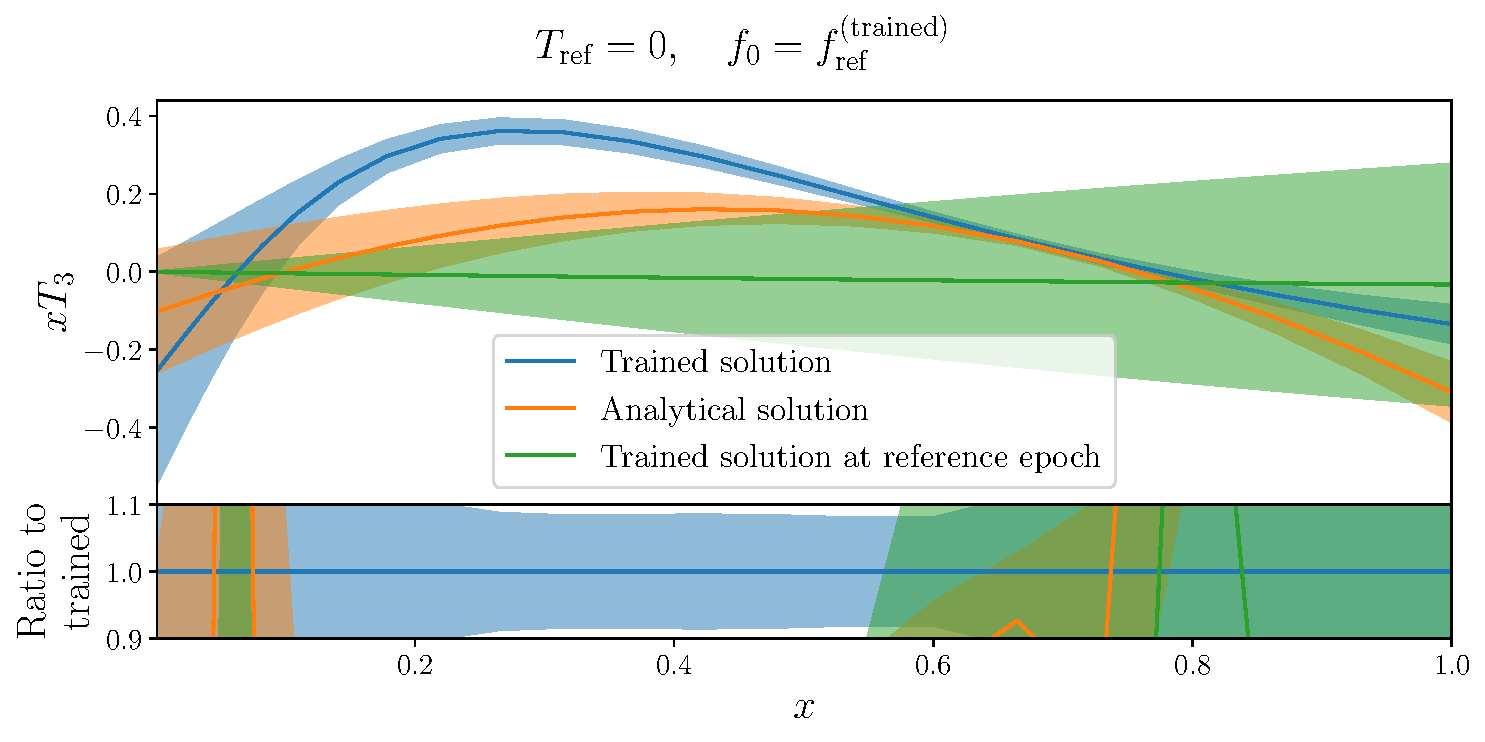
\includegraphics[width=0.48\textwidth]{plots/pdf_plot_ref_0.pdf}
    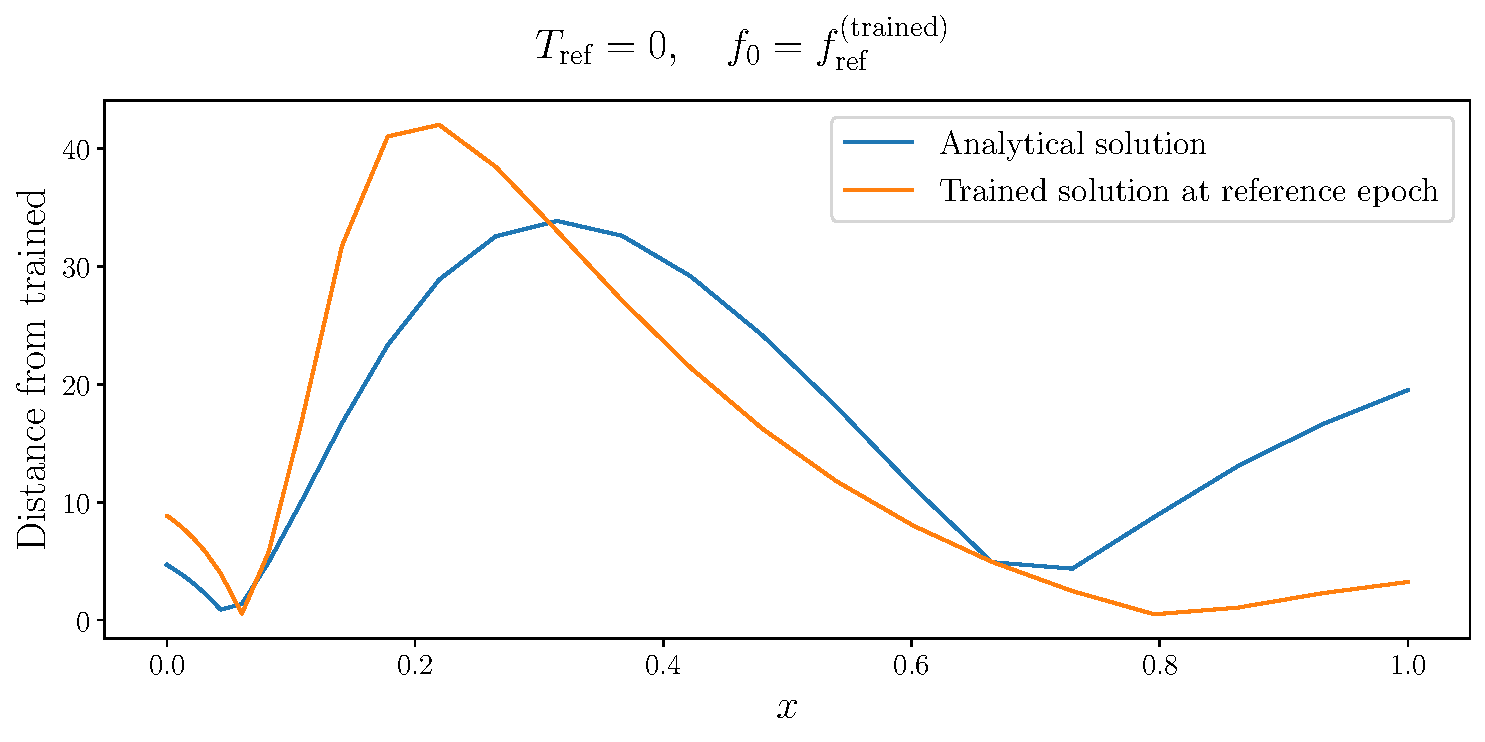
\includegraphics[width=0.48\textwidth]{plots/distance_plot_ref_0.pdf}
    \caption{Same as Fig.~\ref{fig:xT3_analytical_ref}, but for $T_{\rm ref} = 0$.
    \ac{Plots obtained with L2 data}}
    \label{fig:xT3_analytical_ref_0}
  \end{figure}
  % ===================================

  % ===================================
\begin{figure}[t!]
    \centering
    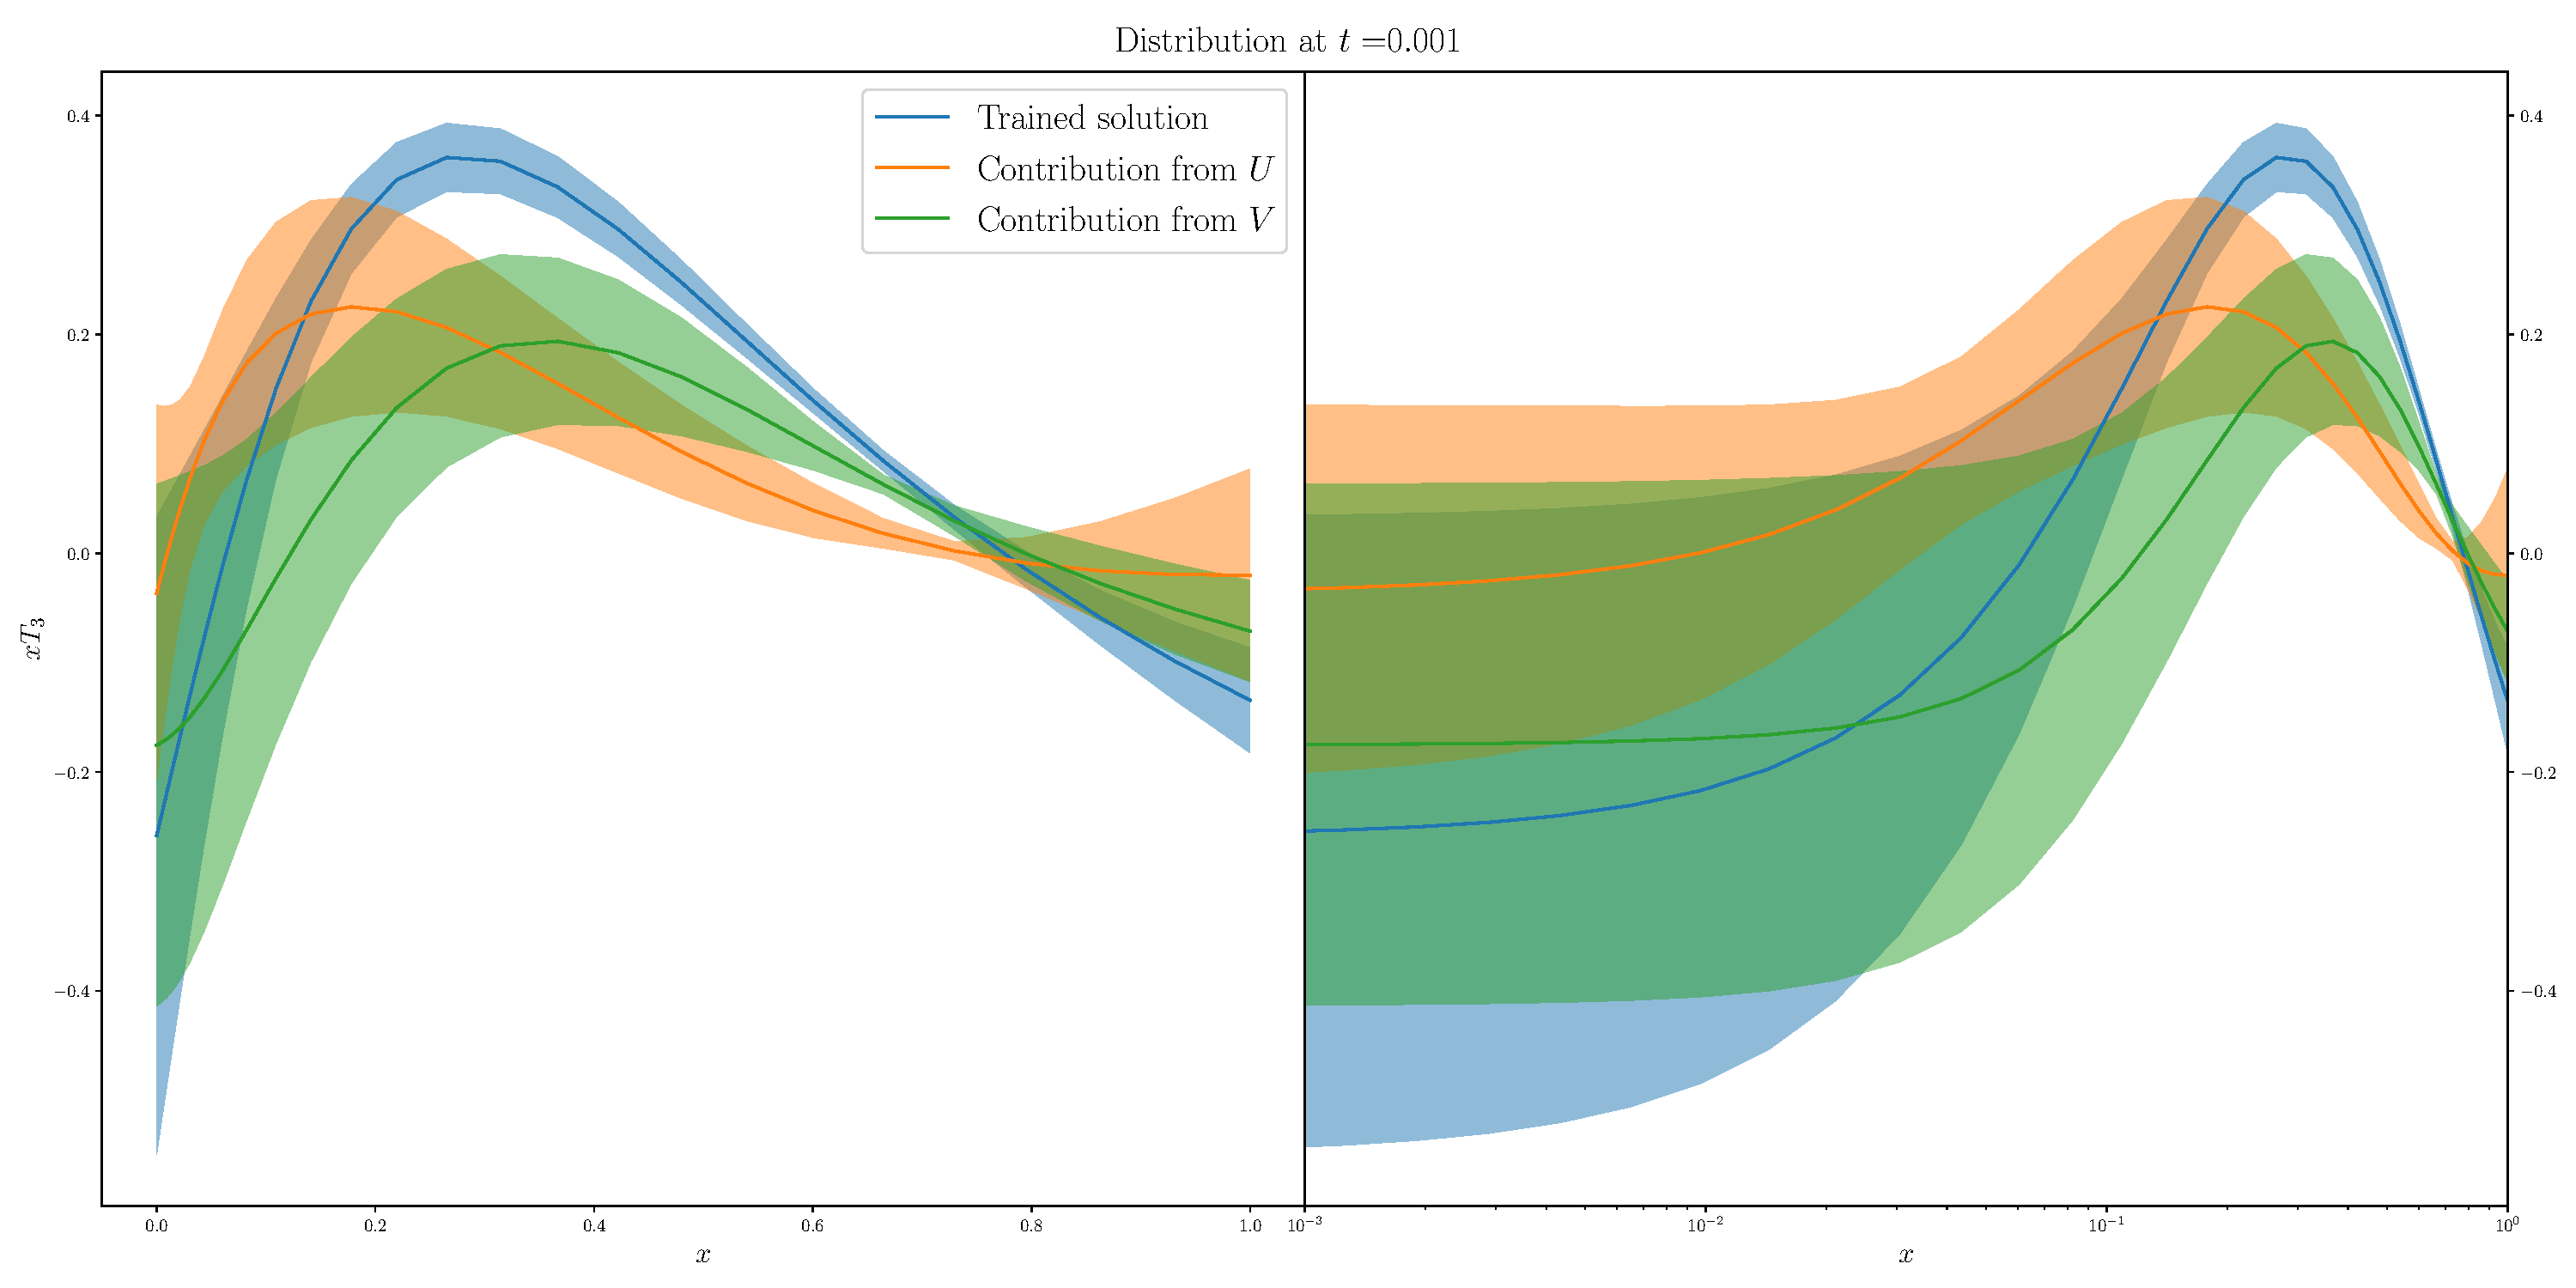
\includegraphics[width=0.65\textwidth]{plots/xT3_u_v_contribution_small_t.pdf}
    \\
    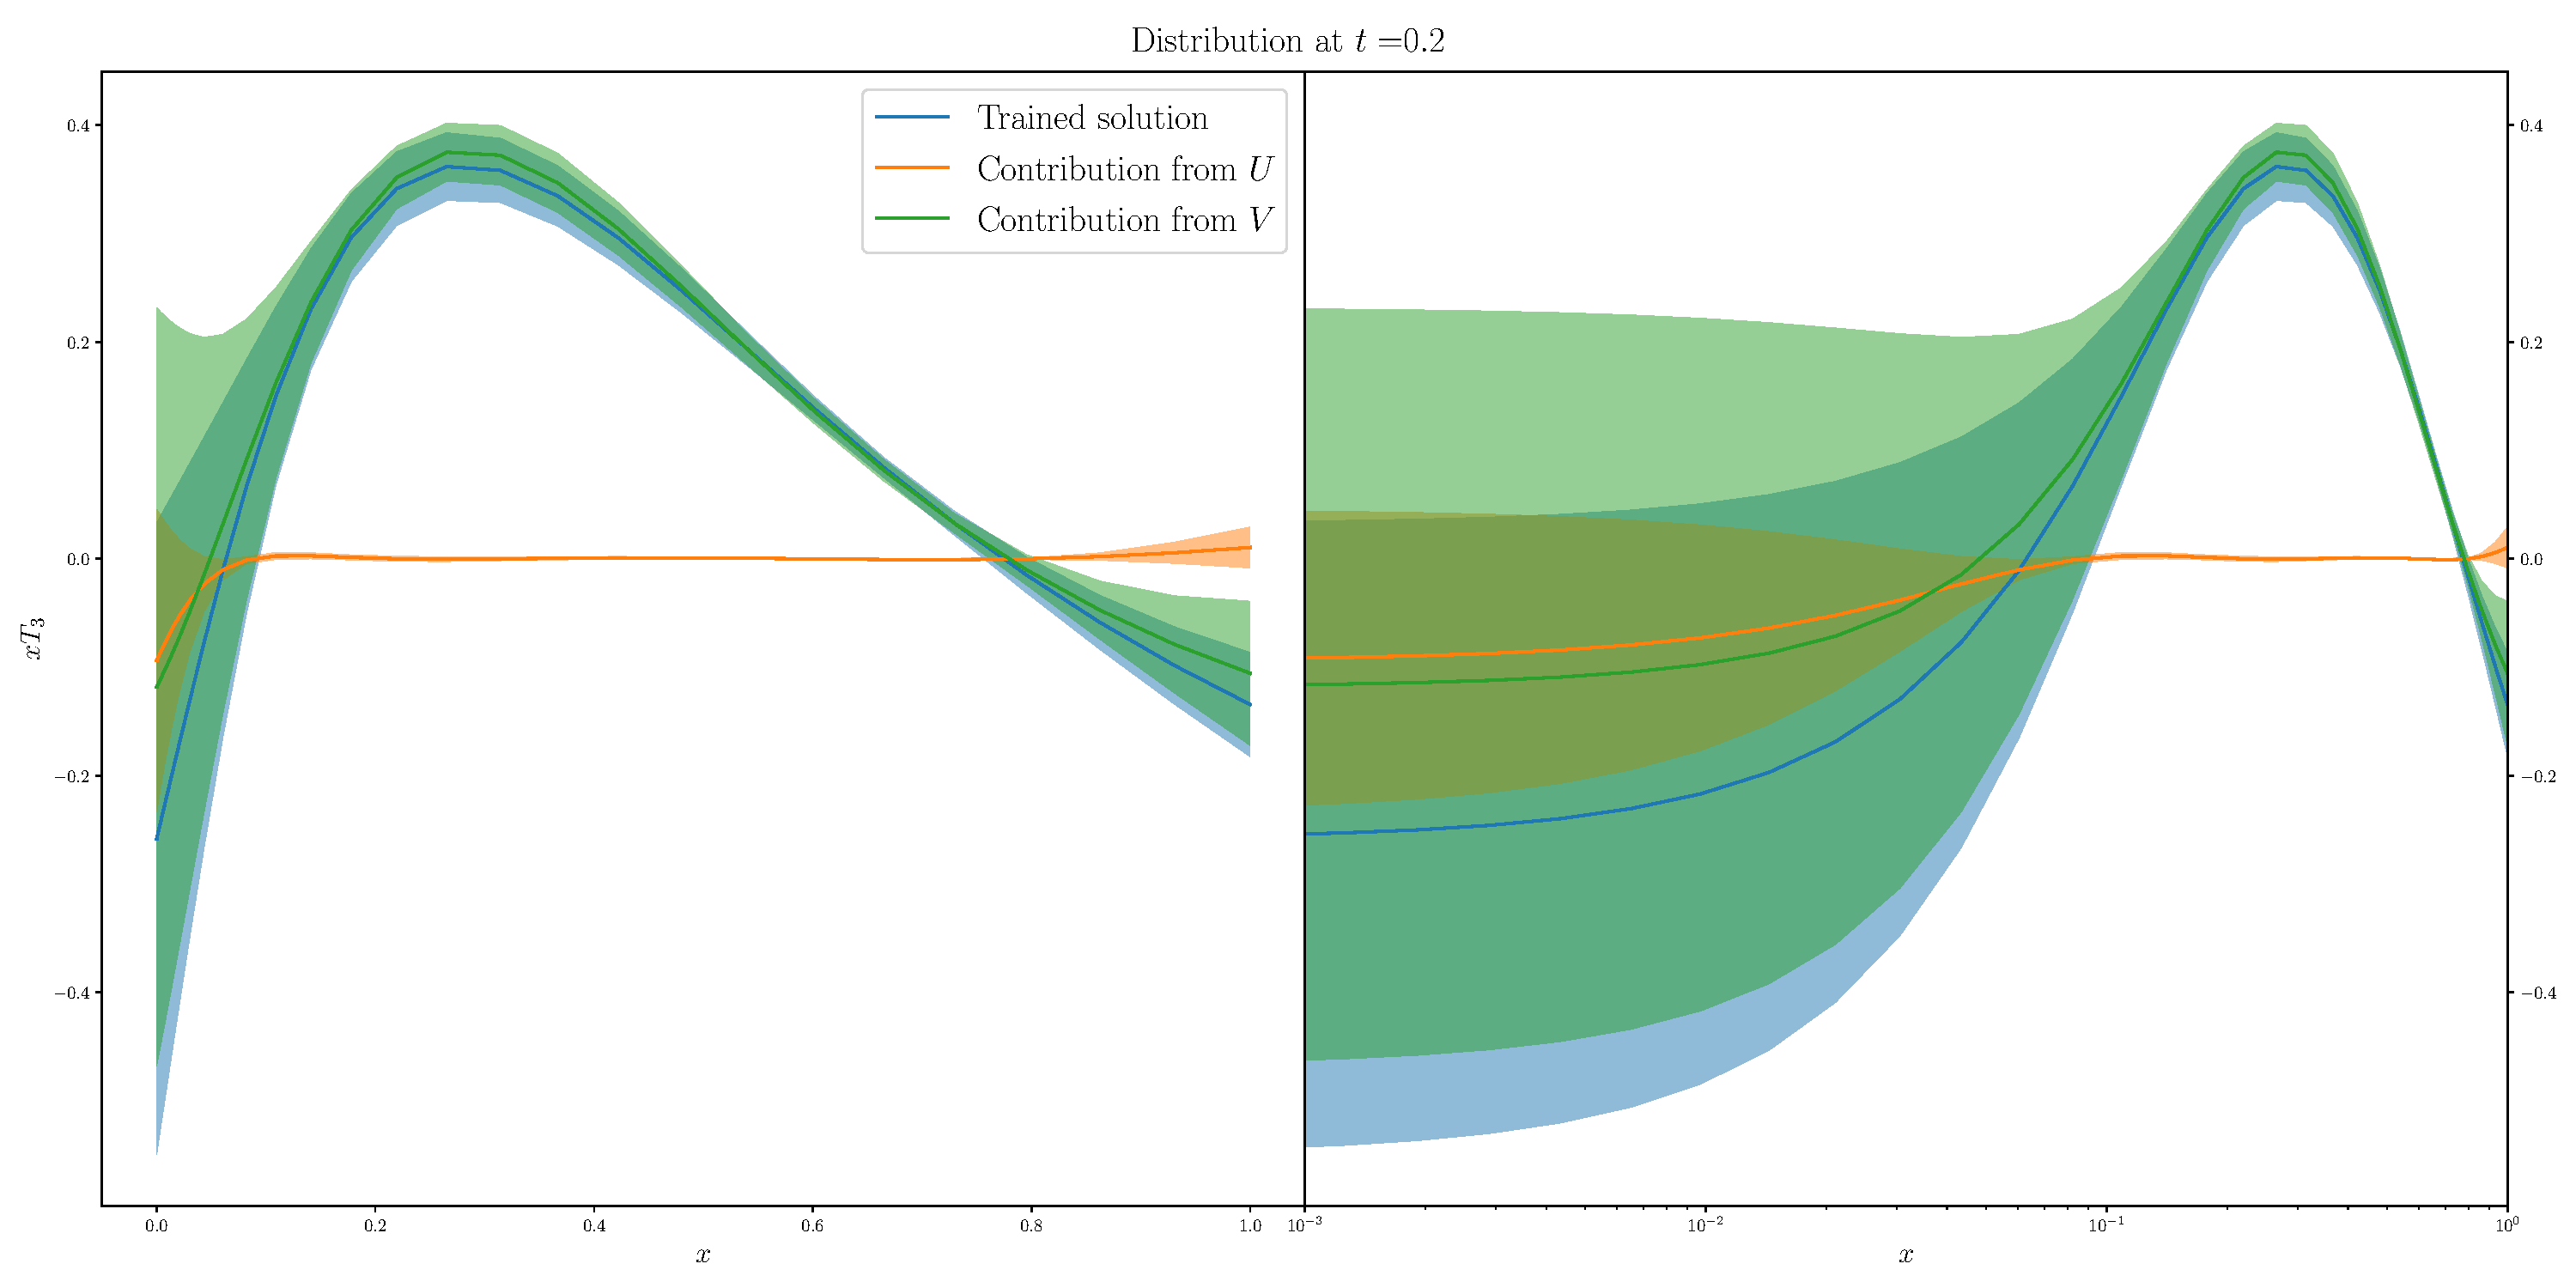
\includegraphics[width=0.65\textwidth]{plots/xT3_u_v_contribution_eot.pdf}
    \caption{Contribution of the $U$ and $V$ terms to the solution. The top panel
    shows this breakdown at early stages of the analytical training ($t=0.001$);
    the bottom panel shows the contributions at the end of training (eot). 
    These plots have been obtained by taking the
    $t_{\rm ref} = 30000$ and $f_0 = f_{t_{\rm ref}}$ using L2 data. \ac{These
    plots will be modified (font size, etc...) to match the other figures.}}
  \end{figure}
  % ===================================
  
  
\FloatBarrier
